\documentclass{article}

\usepackage[utf8]{inputenc}
\usepackage{foar705journal}
\usepackage{subfiles}
\usepackage{minted}
\usepackage{graphicx}
\usepackage{enumitem}

\graphicspath{{./Figures/}}

\newboolean{printCode}
\setboolean{printCode}{true}

\newcommand{\startdeflist}[0]
{\begin{description}[style=unboxed, labelwidth=\linewidth,
font =\sffamily\itshape\bfseries, listparindent =0pt,
before =\sffamily]}

\title{Learning Journal Weeks 9 - 13}
\author{Bree Kelly}
\date{}

\begin{document}

\maketitle

\tablesofcontentsanderrors

\newpage
\section{Tuesday October 15th 2019}

\subsection{Data Carpentry}
\textbf{Intention:} Complete Data Carpentry on R, lessons 3 and 4.

\textbf{Actions:} Following the instructions on the Data Carpentry website, I go through the lessons and answer the following questions:

\subsubsection{Lesson 3: Starting with Data}

\textit{What is a data.frame?}

The representation of data in the format of a table where the columns are vectors that all have the same length. It is a data structure that forms a building template for data. It does the same thing every time. Infrastructure for data.

\textit{How can I read a complete csv file into R?}

Run the function \mintinline{R}|read_csv(filename)|. 

You can also use the function view to see it in the top left pane.

\textit{How can I get basic summary information about my dataset?}

Using functions such as \mintinline{R}|dim()| (no. of rows and columns), \mintinline{R}|nrow()| (no. of rows), \mintinline{R}|ncol()| (no. of columns), \mintinline{R}|head()| (shows first 6 rows), \mintinline{R}|tail()| (shows last 6 rows), \mintinline{R}|names()| (shows column names), \mintinline{R}|str()| (structure of object), and finally \mintinline{R}|summary()| (returns summarised statistics for each column).

\textit{How do I convert between strings and factors?}

Using \mintinline{R}|factor()|

\textit{Describe the difference between a factor and a string.}

I'm not sure about this one.

\textit{Why would I want strings to be treated differently?}

Depends on the type of data analysis you wish to employ and how you what to extract information.

\textit{How do I reorder and rename factors?}

By specifying the factor you wish to rename using \mintinline{R}|[]| with an integer inside and assigning (using an arrow) the new name. To reorder them, you use the assign function, combine function and factor function, eg.

\begin{minted}[breaklines]{R}
memb_assoc <- factor(memb_assoc, levels = c("No", "Yes", "Undetermined"))
\end{minted}

\textit{How do I change how character strings are handled in a data frame?}

Turn them into numerical integers, eg, \mintinline{R}|as.numeric(as.character(year\_fct))|

\itemizederror{No package called Tidyverse}{
\item I started by downloading R and RStudio onto my laptop, then switching to my Surface, on which the CSV file of cleaned SAFI data that I produced in the OpenRefine Data Carpentry Lessons is located.
\item I followed the instructions to download tidyverse in order to use the \mintinline{R}|read_csv()| function, but running \mintinline{R}|library(tidyverse)| returned `Error in library(tidyverse) : there is no package called ``tidyverse."
\item I swear I already downloaded that package, but okay. I go to the Packages tab and search `tidy. No tidyverse package.
\item I click Install and select tidyverse and set it installing.
\item Installation is a success.}

I run \mintinline{R}|library(tidyverse)| again. It returns this:

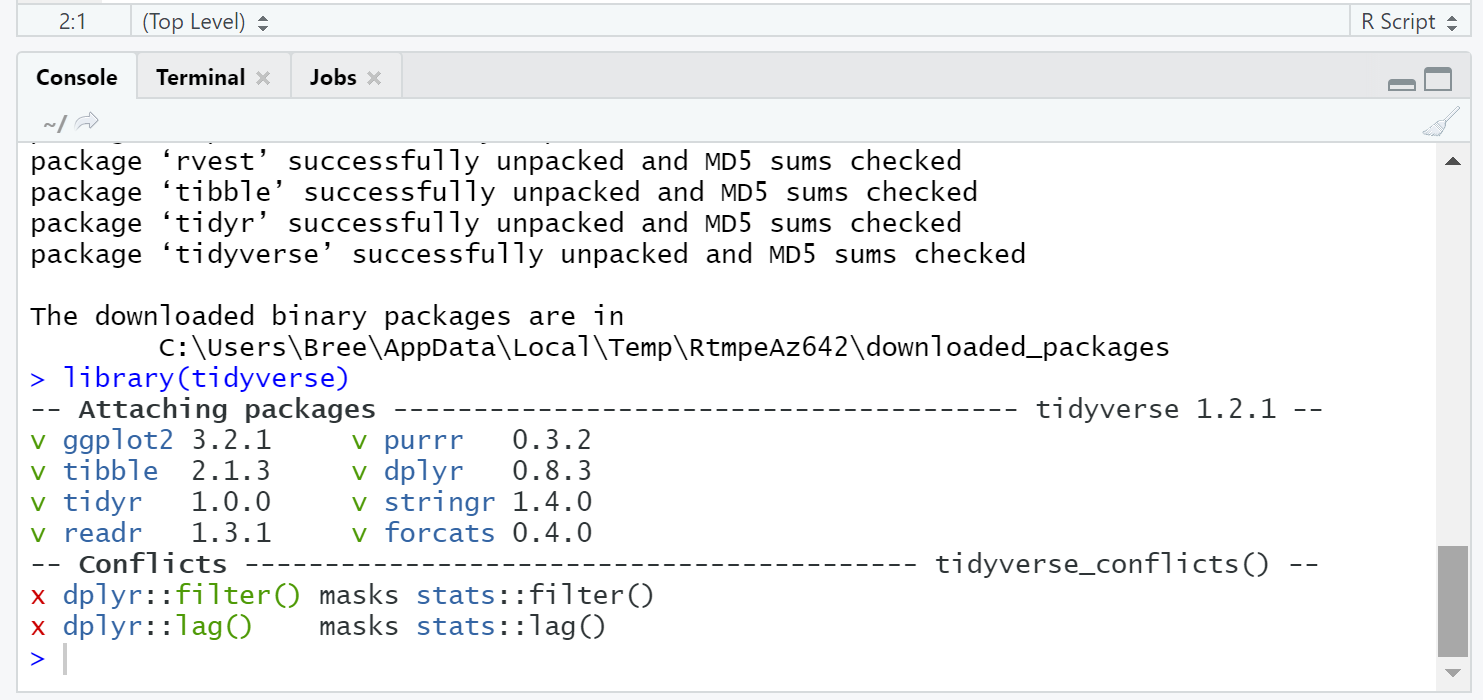
\includegraphics[width=1.0\textwidth]{rstudio_14.PNG}

I copy the CSV file I want to work with (\mintinline{R}|SAFI_clean_exercise_CSV.csv|) into the working directory (Computer/Documents/). I run

\begin{minted}[breaklines]{R}
interviews <- read_csv("SAFI_clean.csv", na = "NULL") 
\end{minted}

 as per the instructions, leaving out the part of the file name I added (ie.\mintinline{R}|_exercise_CSV|) because I am an idiot. Of course, this is returned: Error: unexpected `NULL in
 
\begin{minted}[breaklines]{R}
interviews <- read_cscv("SAFI_clean.csv, na = "NULL")
\end{minted}
 
 I now notice I left out the double quotation mark at the end of the file name, so I correct this, and it finally prints the following:

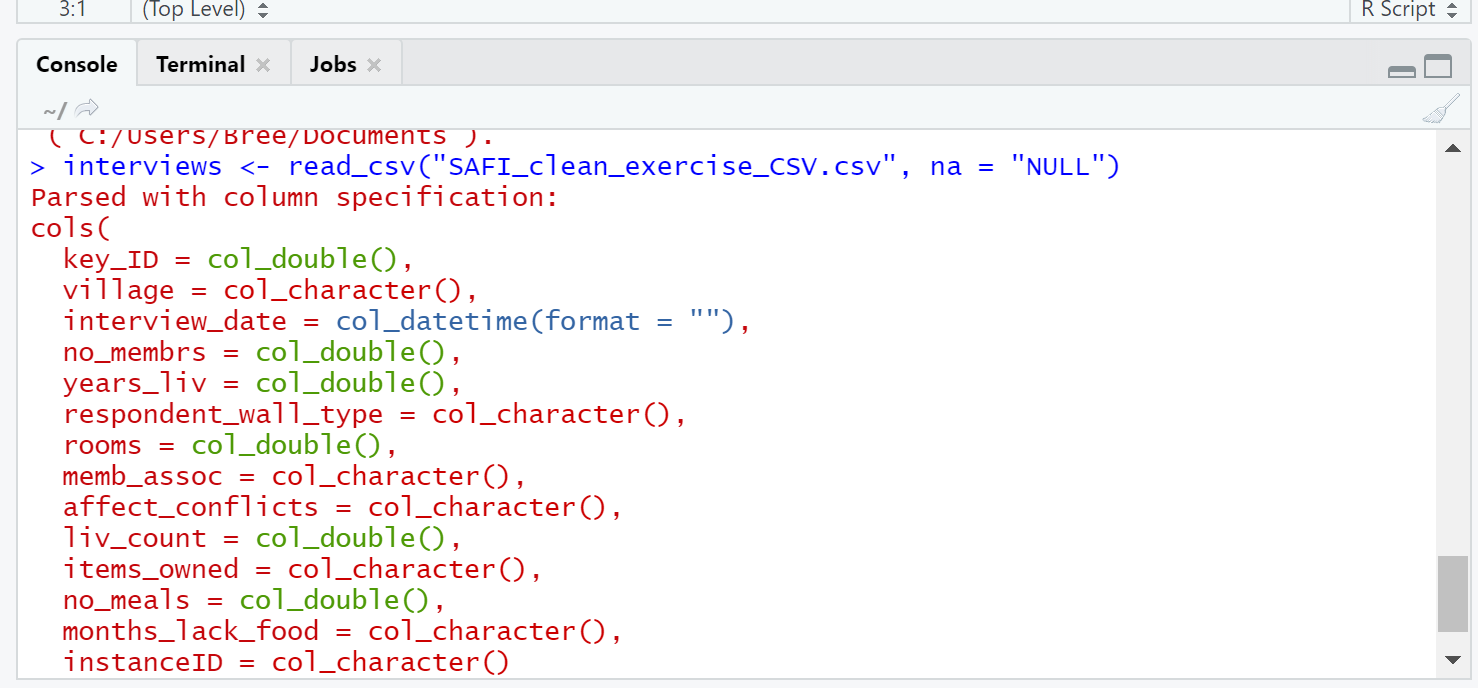
\includegraphics[width=1.0\textwidth]{rstudio_15.PNG}

I can finally move on. I try running just `interviews to see the file:

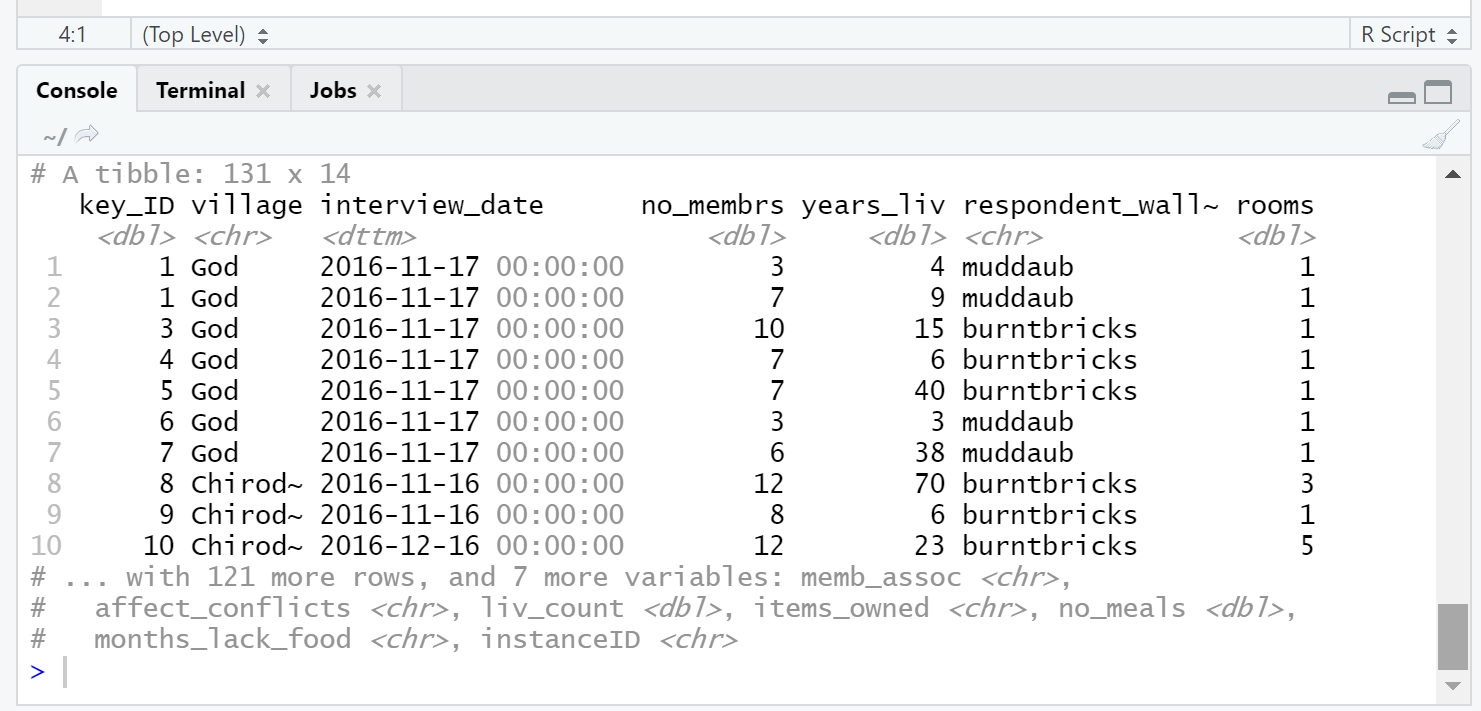
\includegraphics[width=1.0\textwidth]{rstudio_16.PNG}

I then try \mintinline{R}|view(interviews)|, which returns an excel-sheet-looking table in a new tab within the top left pane:

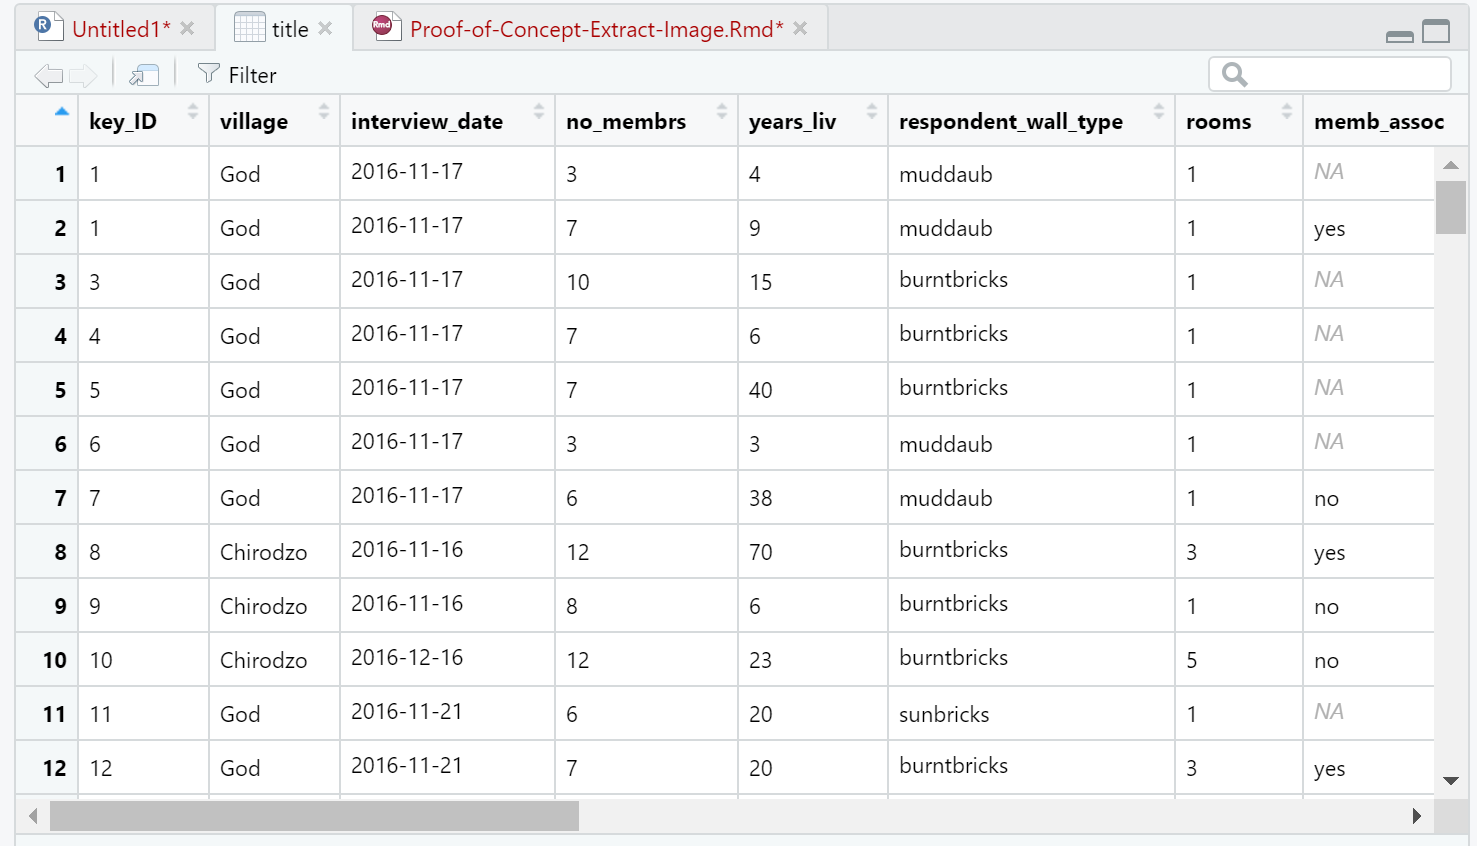
\includegraphics[width=1.0\textwidth]{rstudio_17.PNG}

I then try \mintinline{R}|head(interviews)|, which returns this:

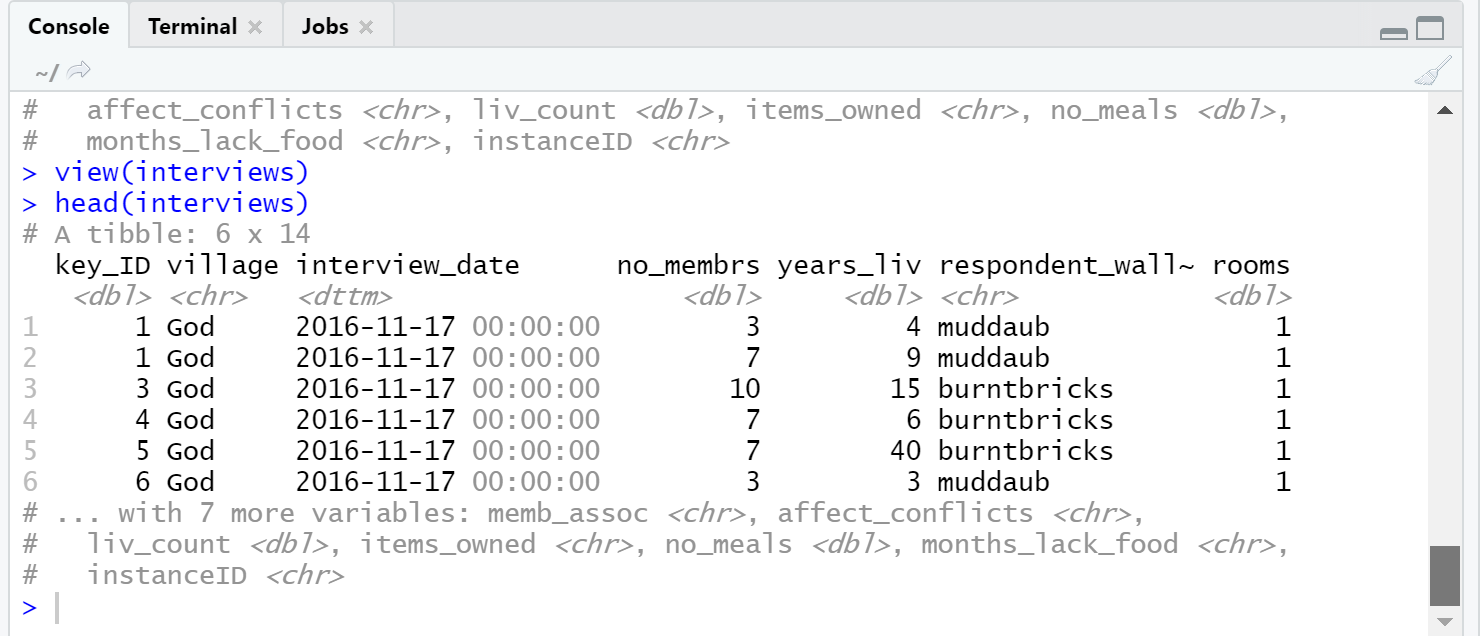
\includegraphics[width=1.0\textwidth]{rstudio_18.PNG}

\itemizederror{Missing Variable?}
{\item (refer to previous section and above images)
\item Not sure how to interpret it, but I didnt get an error for once.
\item I read further into the lesson that \mintinline{R}|head(interviews)| prints the first 6 lines of the file, which appears to be the case when I ran it.
\item I run the various ways to specify columns and rows and such, including \mintinline{R}|interviews[1, 1]|, \mintinline{R}|interviews[1, 6]|, \mintinline{R}|interviews[[1]]|, \mintinline{R}|interviews[1]|, \mintinline{R}|interviews[1:3, 7]|, and \mintinline{R}|interviews[3, ]|.
\item They all run fine, except with the last one, although it executes fine, I can see one difference in the results – instead of \mintinline{R}|8 more variables|, mine states that there are \mintinline{R}|7 more variables|, and appears to be missing the \mintinline{R}|rooms <dbl>|.
\item I can also see a 1 after \mintinline{R}|burntbricks| on my console, which does not appear in the example.
\item Maybe rooms is over there somewhere. I cant figure it out.}

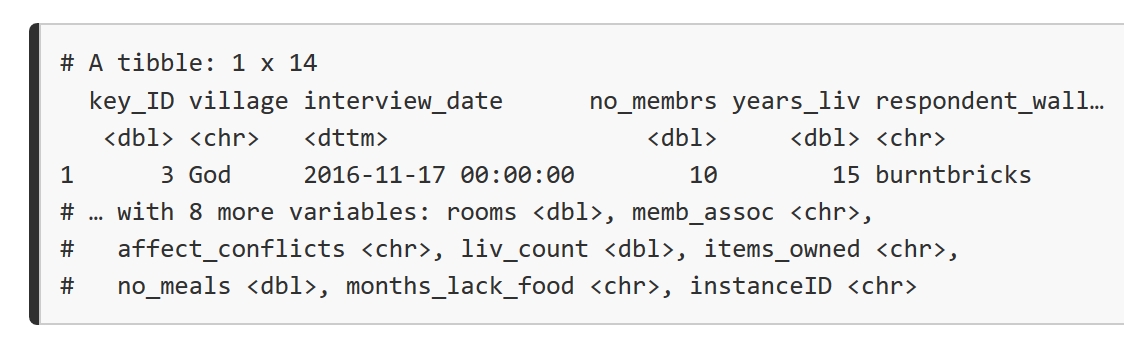
\includegraphics[width=1.0\textwidth]{rstudio_19.PNG}

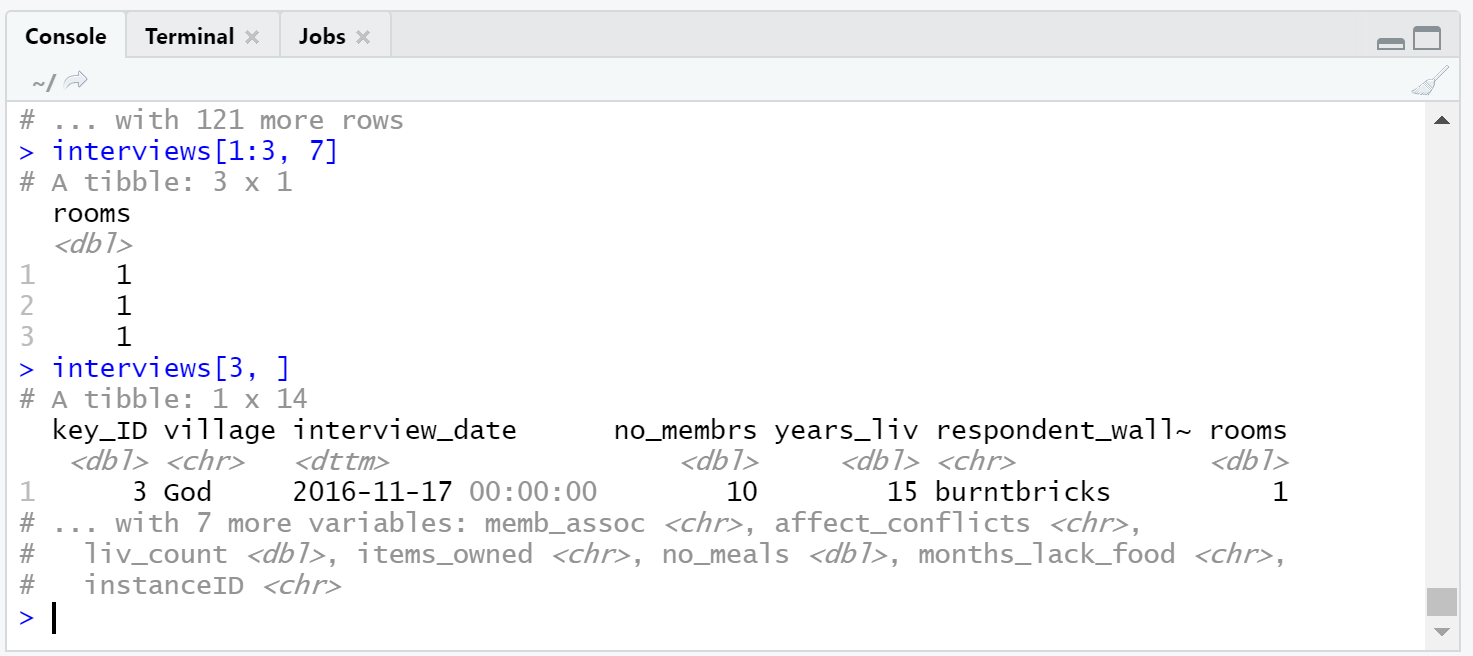
\includegraphics[width=1.0\textwidth]{rstudio_20.PNG}

I tried to complete the following exercise:

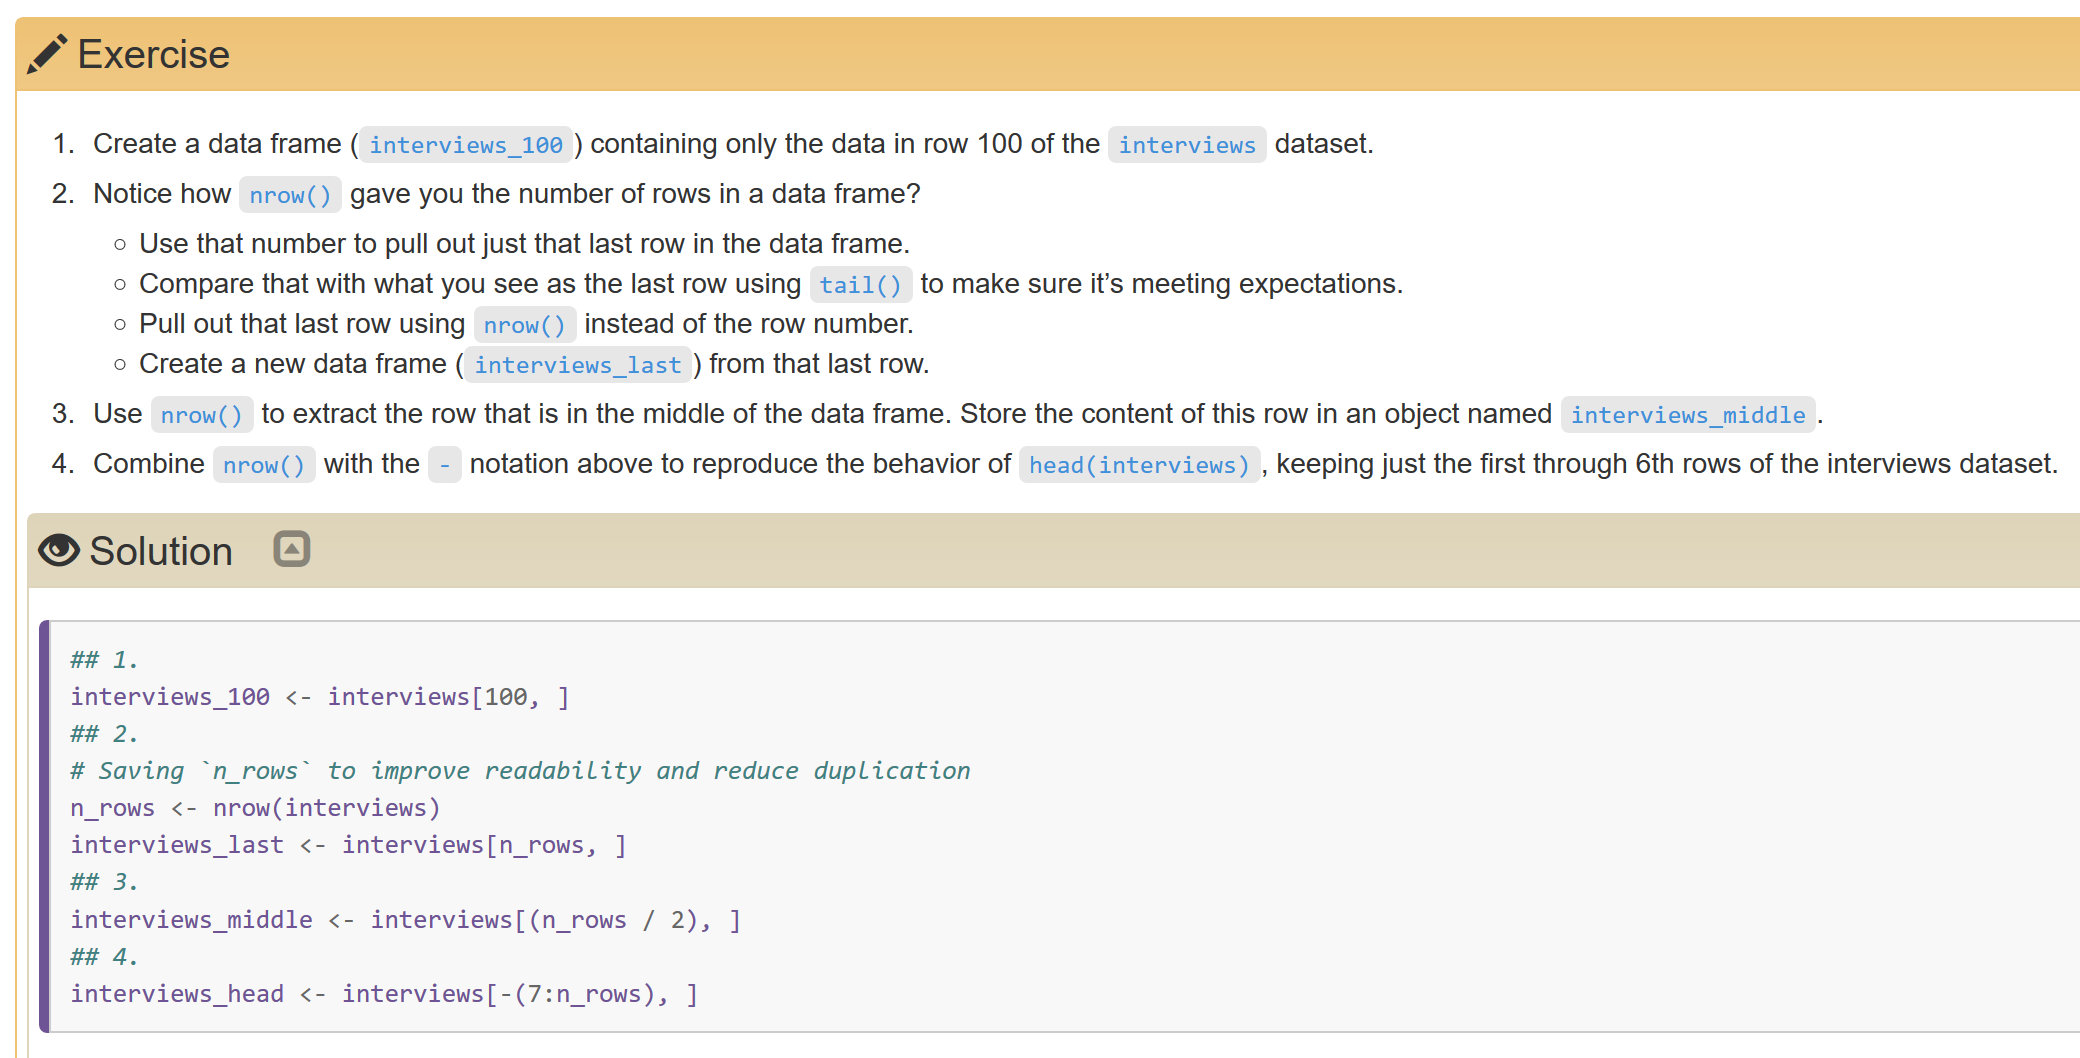
\includegraphics[width=1.0\textwidth]{rstudio_21.PNG}

I did the first part correctly (\mintinline{R}|interviews <- interviews[100, ]|), but got stuck after that. I feel like the instructions are not clear. The second part sounds like its using what you created in the first part, but maybe thats not the case. I tried a few different things, but had to look at the Solution, and even then, I cant fully grasp what is happening in the exercise. I need more help and explanation on this one. Going through the lesson a second time, I think I understand it a little better, but Im still not 100 per cent on vectors, strings, and factors.

\textbf{Result:} Lesson 3 completed (to best of my ability) and recorded in Learning Journal.

\section{Wednesday October 23rd 2019}

\subsection{Data Carpentry}

\subsubsection{Lesson 4: Introducing dplyr and tidyr}

\textbf{Intention}: Complete Data Carpentry on R, Lesson 4.

\textbf{Action}: Following the instructions on the Data Carpentry website, I go through the lessons and answer the following questions:

\textit{How can I select specific rows and/or columns from a data frame?}

Select(data frame, column name, column name, column name)

`To select columns of a data frame, use \mintinline{R}|select()|.

The first argument to this function is the data frame (\mintinline{R}|interviews|), and the subsequent arguments are the columns to keep.

To be more specific, use \mintinline{R}|filter|:

\mintinline{R}|filter(data frame, column name == "column component")|

\textit{How can I combine multiple commands into a single command?}

There are three ways to combine commands.
Intermediate steps, nesting, and pipes.
Intermediate steps works, but is messy.
Nesting is ‘neater,’ but can become difficult to keep track of things.
Pipes is the preferred method.

Exercise – my answer: 

\begin{minted}[breaklines]{R}
interviews_members <- interviews %>%
filter(memb_assoc == "yes") %>%
select(affect_conflicts, liv_count, no_meals)
\end{minted}

\itemizederror{Understanding Filter Function}
{\item Checking solution, I see that I got this down pat.}

\mintinline{R}|interviews_god <- select(filter(interviews, village == "God"), no_membrs, years_liv|

I don’t understand the break down of this construction. \mintinline{R}|filter| acts on 
\mintinline{R}|interviews| as the data frame, but what data frame does \mintinline{R}|select work| on in order to also select \mintinline{R}|no_members| and \mintinline{R}|years_liv| ?

\textit{How can I create new columns or remove existing columns from a data frame}?
Using the \mintinline{R}|mutate| function, you can add a column by using information in other columns.
In the exercise, I got an answer that was close, but in the wrong order:

\begin{minted}[breaklines]{R}
interviews_village <- interviews %>%
select(village) %>%
mutate(total_meals = no_members*no_meals) %>%
select(total_meal > 20)
The correct answer was:
interviews_village <- interviews %>%
mutate(total_meals = no_membrs * no_meals) %>%
filter(total_meal > 20) %>%
select(village, total_meals)
\end{minted}

I realised after trying it out that it should be \mintinline{R}|no_membrs|, not \mintinline{R}|no_members|, and I made a typo when writing \mintinline{R}|total_meals| (I left off the s).
After fixing these small issues, it worked fine.

\textit{How can I reformat a dataframe to meet my needs}?

Reshaping by gathering and spreading – creating new tables using variables and values within the original data frame.

\itemizederror{Mismatch between Data Carpentry and RStudio}
{\item When completing the exercise for this, I copied the instructions directly into RStudio, and I couldn’t see the correlation between what I was seeing in RStudio and on the Data Carpentry website.
\item It indicated that a separate new table would be created with 4 rows, but it appeared to just add them onto the end of the existing table:

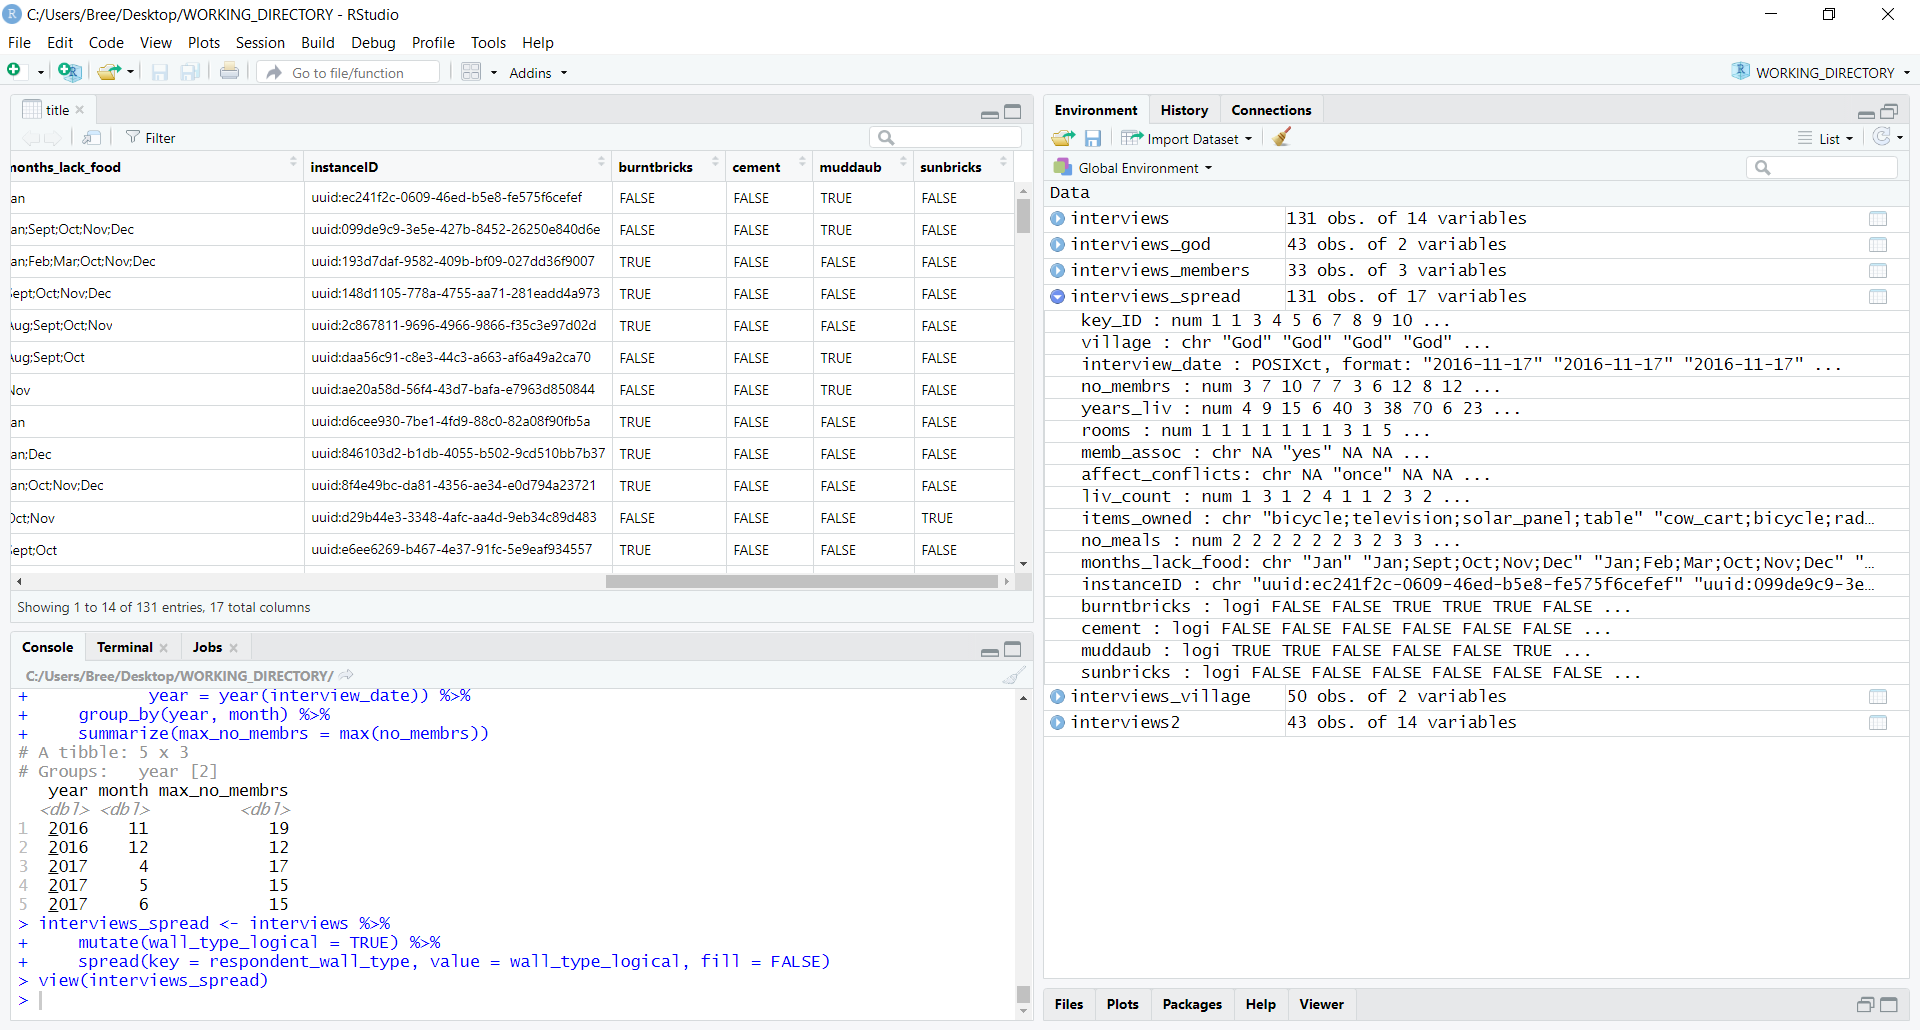
\includegraphics[width=1.0\textwidth]{rstudio_22.PNG}

This seems to be how it’s supposed to work, but I’m not fully wrapping my head around the concept. The highlighted line is the one I’m having trouble understanding:

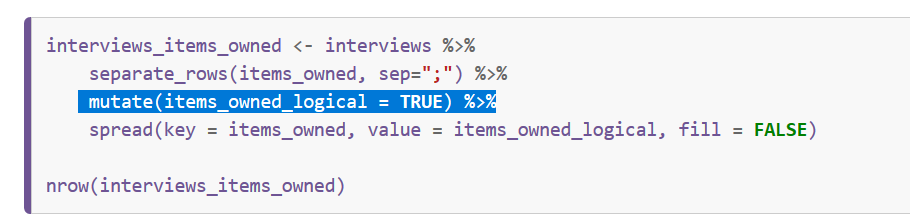
\includegraphics[width=1.0\textwidth]{rstudio_23.PNG}}

\itemizederror{NA vs /}
{\item The exercise going through the Applying \mintinline{R}|spread()| to clean our data process states that the last column in the data frame after running }

\begin{minted}[breaklines]{R}
interviews_items_owned <- interviews
separate_rows(items_owned, sep=";")  %>%\end{verbatim}
mutate(items_owned_logical = TRUE)  %>%\end{verbatim}
spread(key = items_owned, value = items_owned_logical, fill = FALSE)’
\end{minted}

is / and that it needs to be renamed to be called `NA', but mine is already called that:

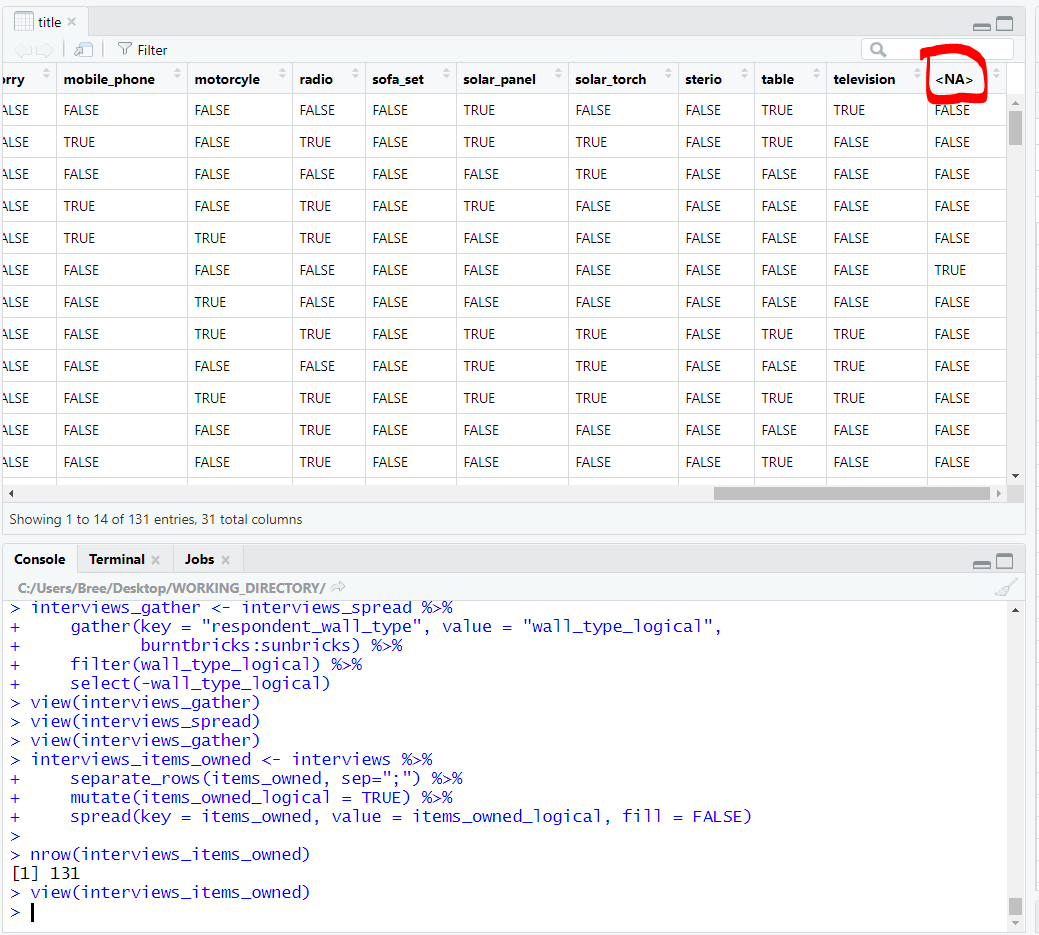
\includegraphics[width=1.0\textwidth]{rstudio_24.PNG}

Reading further on, after running

\begin{minted}[breaklines]{R}
interviews_items_owned <- interviews_items_owned %>%
rename(no_listed_items = <NA>)
\end{minted}

to rename the column, I see it has replaced the NA with \mintinline{R}|no_listed_items|.

Perhaps it was just showing NA before because the value was NA, and the Data Carpentry site just expected the value of NA to be shown as /.

\itemizederror{Lack of Explanation}
{\item We haven’t really got an explanation for the \mintinline{R}|rowSums| function and the `. in the following argument:

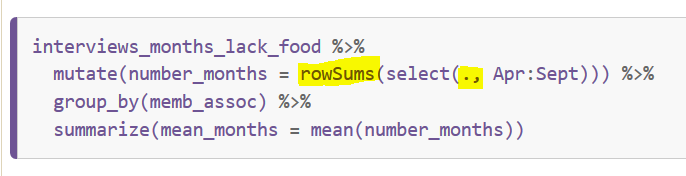
\includegraphics[width=1.0\textwidth]{rstudio_25.PNG}

\item I wrote the final data frame to a csv file then opened the file in Excel to inspect it. \item Success.}

\textbf{Result}: Lesson 4 is complete, and questions are prepared for consultation hour. Next task: complete ‘Lesson 5: Data Visualisation with ggplot2.’

\section{Thursday October 24th 2019}

\subsection{Data Carpentry}

\textbf{Intention}: Complete final lesson for Working with R for Social Scientists: Data Visualisation with ggplot2.

\subsubsection{Lesson 5: Data Visualisation with ggplot2}

\textbf{Actions}: Working through the instructions on the Data Carpentry site, I finish the last lesson for R, answering the following questions:

\textit{What are the components of a ggplot?}

Source data, mapping, variable, geoms, x-axis, y-axis, layers (using + sign), transparency, aesthetics

\mintinline{R}|ggplot(data = <DATA>, mapping = aes(<MAPPINGS>)) +  <GEOM_FUNCTION>()|

\textit{How do I create scatterplots, boxplots, and barplots?}

Scatterplots - \mintinline{R}|geom_point()|

In completing the exercise by myself, I got the basics right, but mixed up the y- and x- axes:

\begin{minted}[breaklines]{R}
ggplot(data = interviews_plotting, aes(x = no_membrs, y = respondent_wall_type)) + geom_jitter(aes(color = respondent_wall_type), alpha = 0.5)
\end{minted}

Should have been
\begin{minted}[breaklines]{R}
ggplot(data = interviews_plotting, aes(x = village, y = rooms)) + geom_jitter(aes(color = respondent_wall_type))
\end{minted}

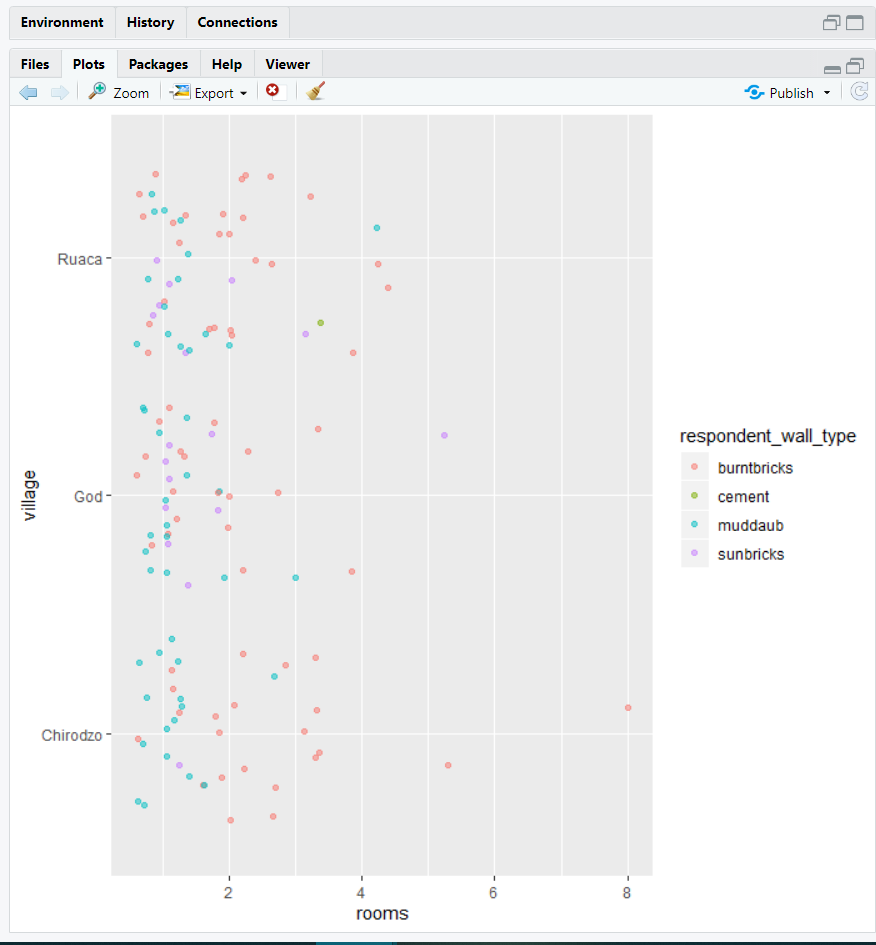
\includegraphics[width=1.0\textwidth]{rstudio_26.PNG}

Boxplots- \mintinline{R}|geom_boxplot()|

\itemizederror{Change Boxplot to be in front of jitter?}
{\item What do you need to change in the code to put the boxplot in front of the points such that it’s not hidden?
\item I tried a number of things, including switching the order of the \mintinline{R}|boxplot| and \mintinline{R}|jitter|, but this came up with an error. I also tried switching around the alpha values, that did not work. A question for consultation hours.}

Barplots- \mintinline{R}|geom_line()|

In the \mintinline{R}|barplot| exercise, I used \mintinline{R}|filter(memb_assoc != "NA")| based on the example given, rather than \mintinline{R}|filter(!is.na(memb_assoc))| in the Solution, but I still appeared to produce the same result.

\textit{How can I change the aesthetics (ex. colour, transparency) of my plot?}

\mintinline{R}|aes(alpha = ) aes(color = )|

\textit{How can I create multiple plots at once?}

Faceting: `allows the one plot to be split into multiple plots based on a factor included in the dataset.’

\underline{Exercise}: \textit{Experiment with at least two different themes. Build the previous plot using each of those themes. Which do you like best?}

I actually liked \mintinline{R}|theme_bw()| the best. I tried the dark theme, it was not overly clear or easy to read, but looked cool and moody.

\itemizederror{Customistation?}
{\item For the final exercise where it asks you to play around a bit with customisation and colours, I followed the}
\begin{verbatim}http://docs.ggplot2.org/current/ggtheme.html\end{verbatim}
link and tried this section:

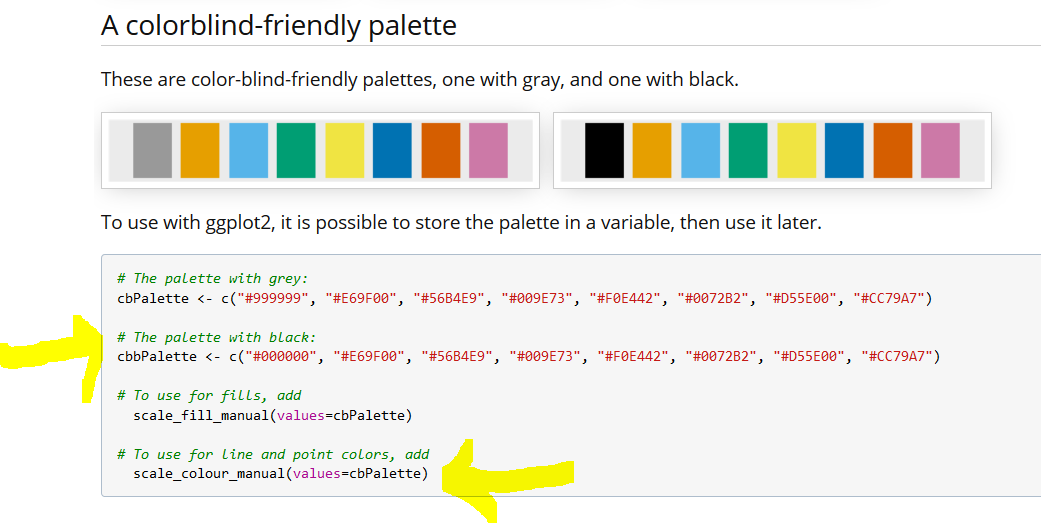
\includegraphics[width=1.0\textwidth]{rstudio_27.PNG}

It wrote this

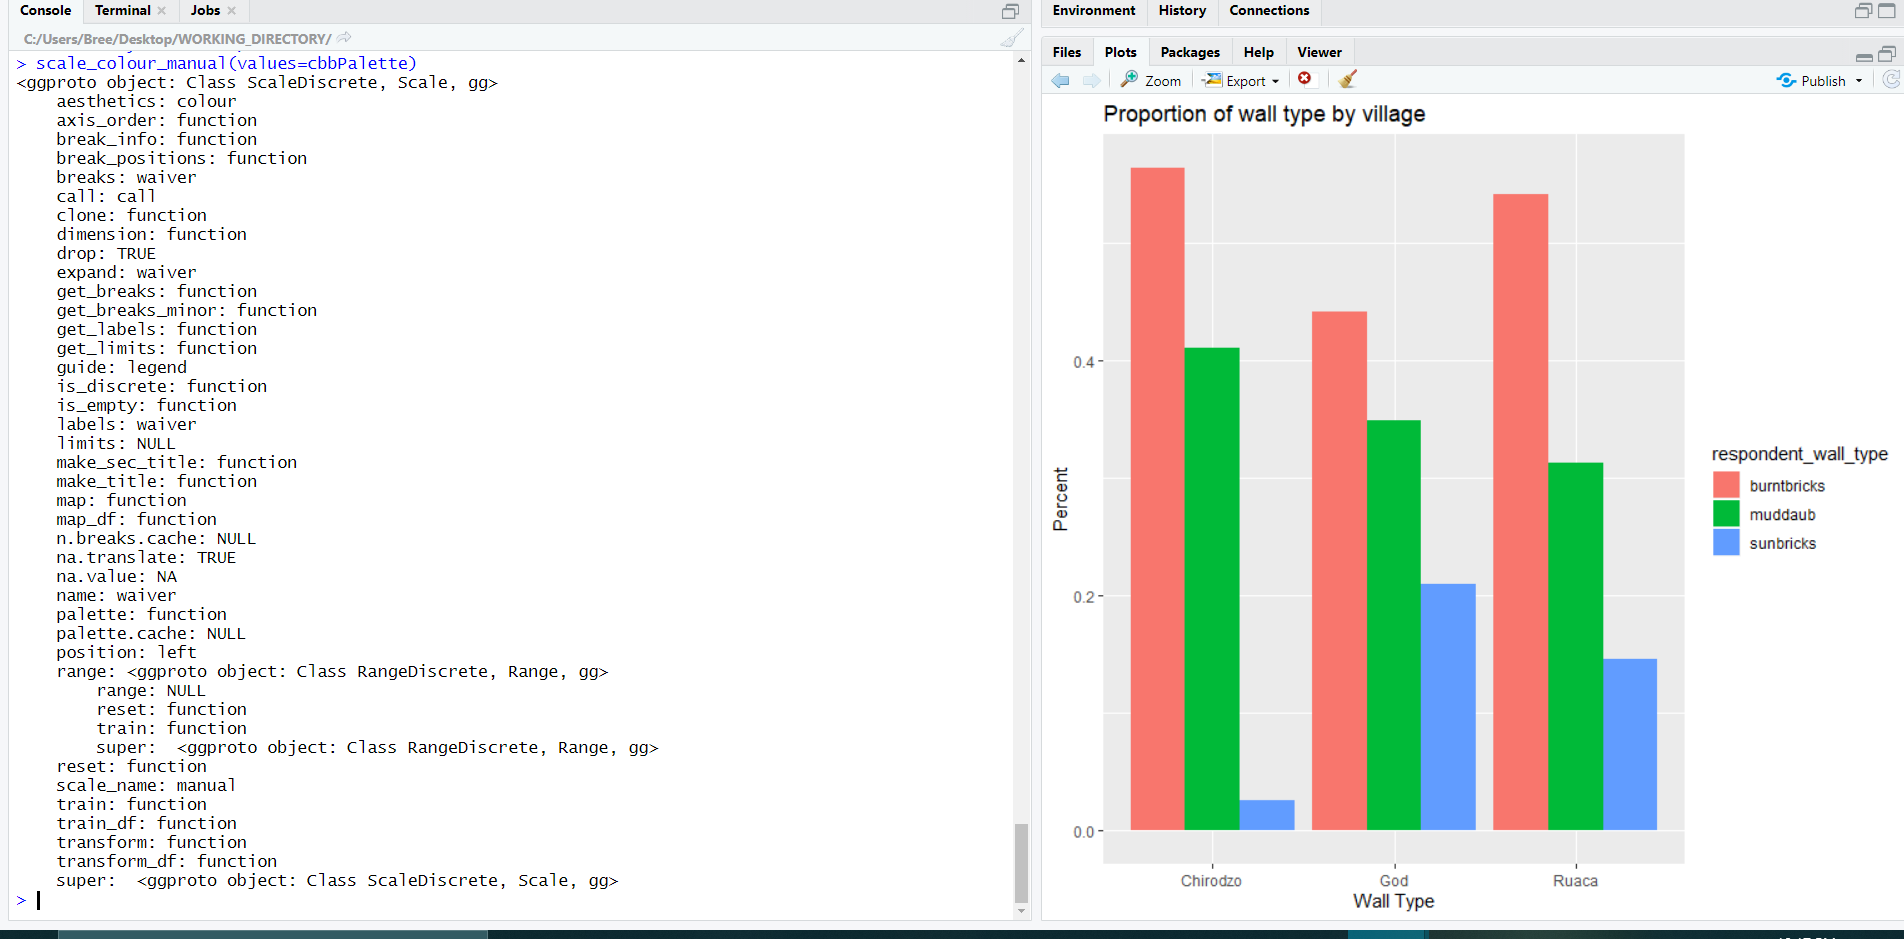
\includegraphics[width=1.0\textwidth]{rstudio_28.PNG}

I’m not sure what this means, but no errors came up(?)

Successfully saved my plot as a png in the \mintinline{R}|fig_output| folder using \mintinline{R}|ggsave()|.

\textbf{Result}: Data Carpentry lessons for R for Social Scientists completed and documented.

\underline{Notes}: I have been using Word due to inability to effectively use OverLeaf, in light of time constraints. I will be meeting with Brian next Wednesday, so I will hopefully be able to work through data recovery and OverLeaf stuff then. (Update: Brian helped me transfer my text into Overleaf for uploading later for marking - 1-11-19).

\subsection{Duplicati - Data Recovery}

\textbf{Intention}: Establish data recovery plan using Duplicati. I have realised that the original setup I had using this method backed my files up onto my laptop itself. If my laptop were to be stolen or run over by a truck, it would all be gone. I need a Cloud-based save destination. I have a Microsoft One Drive, so maybe I can use that.

\textbf{Acitons}: Opening Duplicati 2, I delete my previous attempts at configuring data back up for my FOAR705 folder on my laptop.

\itemizederror{Cannot Setup Cloud-Based Backup}
{\item I start to set up a new one, selecting One Drive as my save method, but cannot proceed past this screen:}

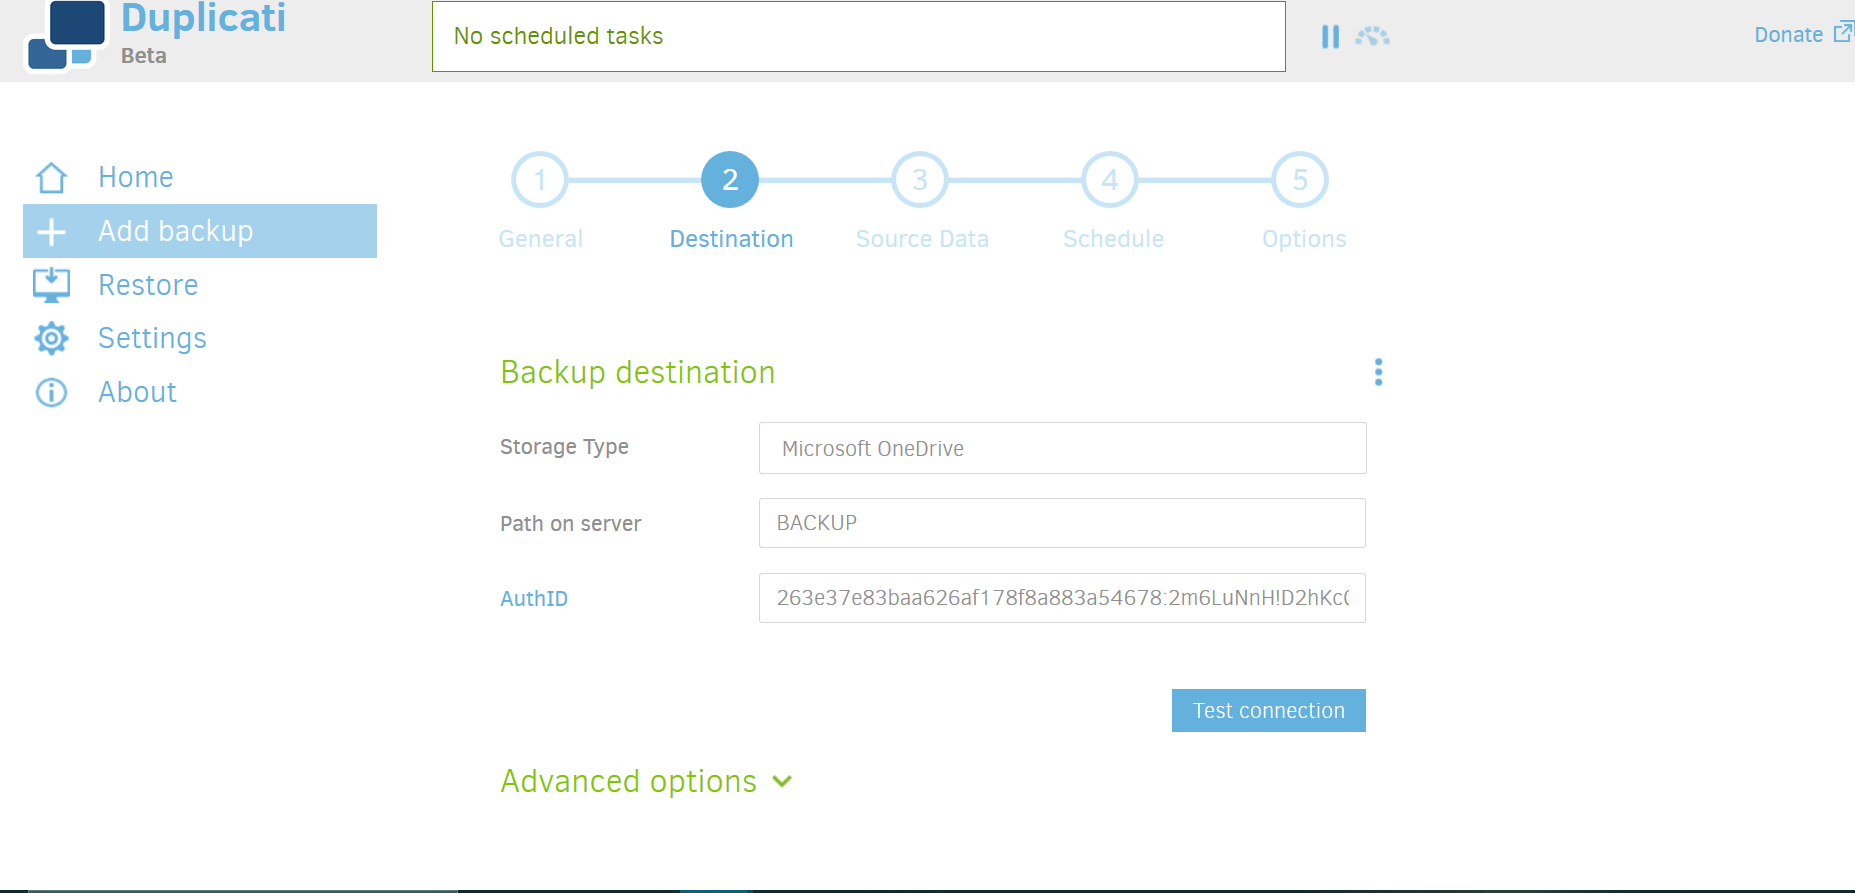
\includegraphics[width=1.0\textwidth]{duplicati_31.PNG}

I just get this error when testing connection: 

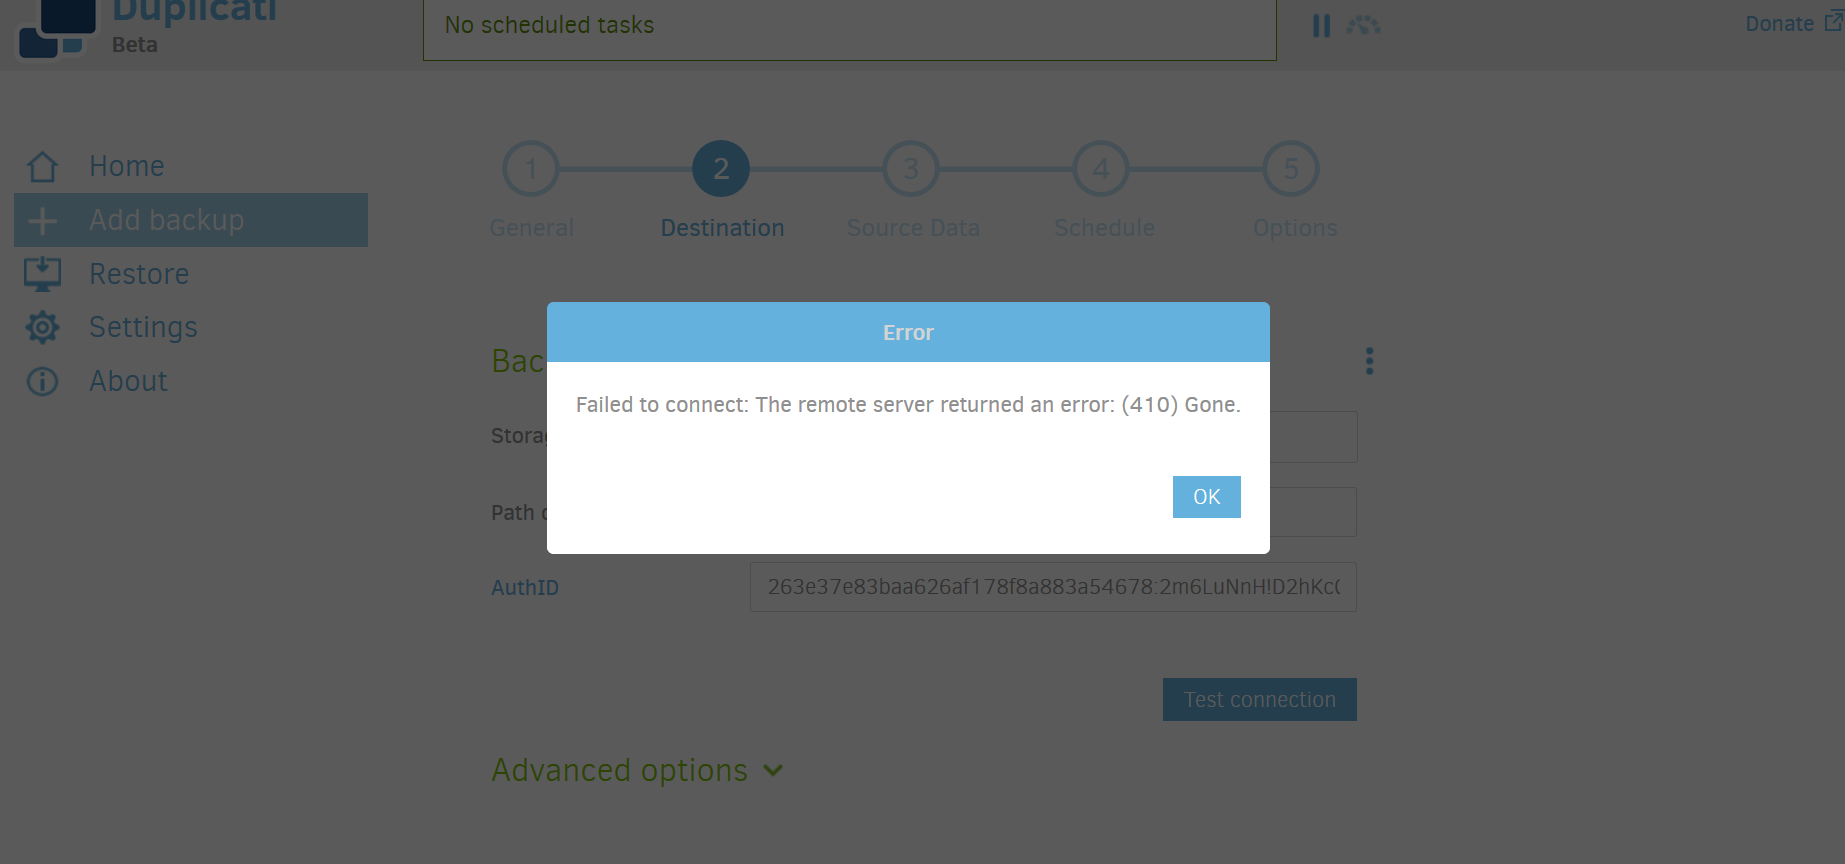
\includegraphics[width=1.0\textwidth]{duplicati_32.PNG}

Despite following these instructions:

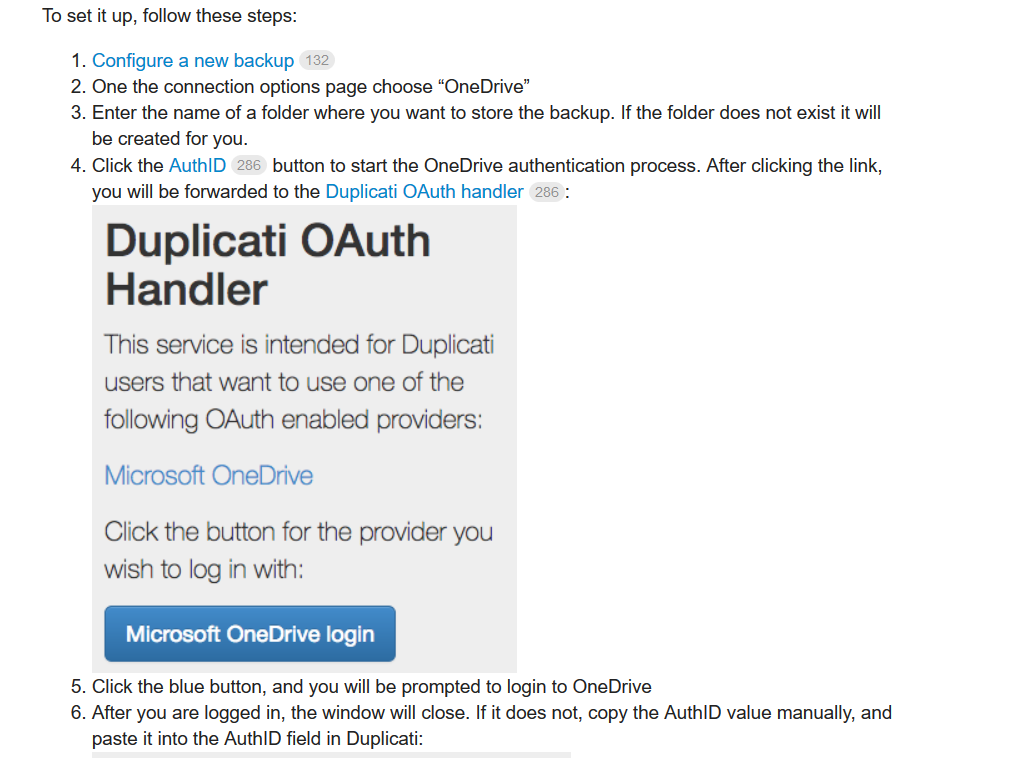
\includegraphics[width=1.0\textwidth]{duplicati_33.PNG}

From this website: 
\begin{verbatim}https://forum.duplicati.com/t/setting-up-onedrive-personal/588\end{verbatim}

It says my page should look like this

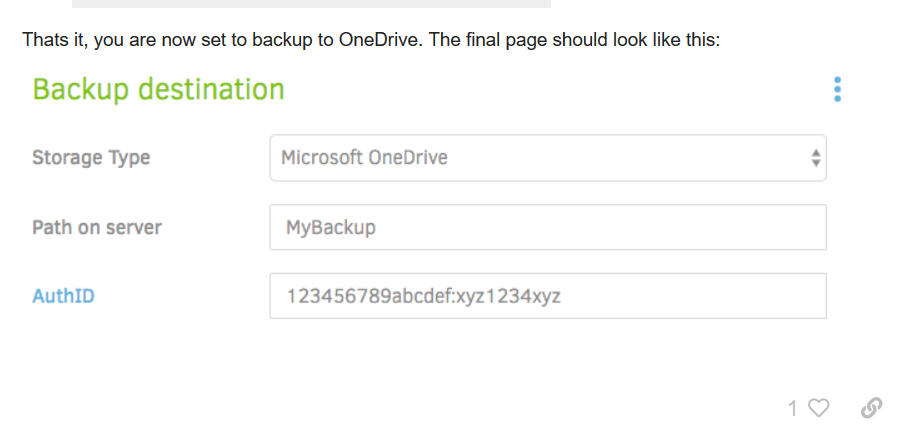
\includegraphics[width=1.0\textwidth]{duplicati_34.PNG}

Which it does. But still error 410. I have sent a Slack message to Brian and will ask tomorrow at consultation hours.

\textbf{Result}: Duplicati partially set up again. Learning journal uploaded to CloudStor 24/10/19 as pdf.

\section{Friday October 25th 2019}

\subsection{Duplicati - Data Recovery}

\textbf{Intention}: Set up multiple configurations for multiple destinations for my FOAR705 files.

\textbf{Actions}: In class, we were guided through the process of setting up a backup configuration using CloudStor as our online server. After class, Brian helped me create an additional backup configuration for backing up to my OneDrive (Microsoft) account.

\itemizederror{Wrong Version of OneDrive}{
\item Initially we could not get the connection to work, and kept getting 'Error 410: Gone'
\item Looking up the issue online and consulting an online forum, we changed the Version of the OneDrive selected and it suddenly worked. Huzzah.}

\textbf{Result}: Files successfully set up to be backed up every night to two online destinations. Organised to demonstrate data recovery next week with Brian. (Update: data recovery was successful. at first, I didn't realise I had to save a file of the configuration and send it to myself via email, but after seeing how this is done, the process made sense. 30-10-19)

\section{Thursday October 31st 2019}

\subsection{Proof of Concept R Scripts}

\subsubsection{Extract Source Images}

\textbf{Intention}: Develop R script that can parse a YAML file into RStudio, extract the information that pertains to the PNG file contained within said YAML file, convert it from the Base64 language in which it is encoded, and then write it to a PNG file.

\textbf{Actions}: Using RStudio, I follow some R Documentation guides, along with advice from Brian to develop the code function by function.

First, I need to parse the YAML file. I have named the YAML file `extract-source-images.yml.' In order to work with YAML files within RStudio, I need to load the YAML package. I do so by downloading it from the Packages tab in the "Files" pane (bottom right). In order to parse the file in RSTudio I will need to use the function \mintinline{R}|yaml.load_file()|.

\mintinline{R}|yaml.load_file(file.path("data","extract-source-images.yml"))|

This code works!

Next, I need to extract some info from within the file.

The HI Workbench project I exported as a YAML file has no Gardiner Codes in it, but it does have two image files, called `wall\_photo' and `line\_drawing.'

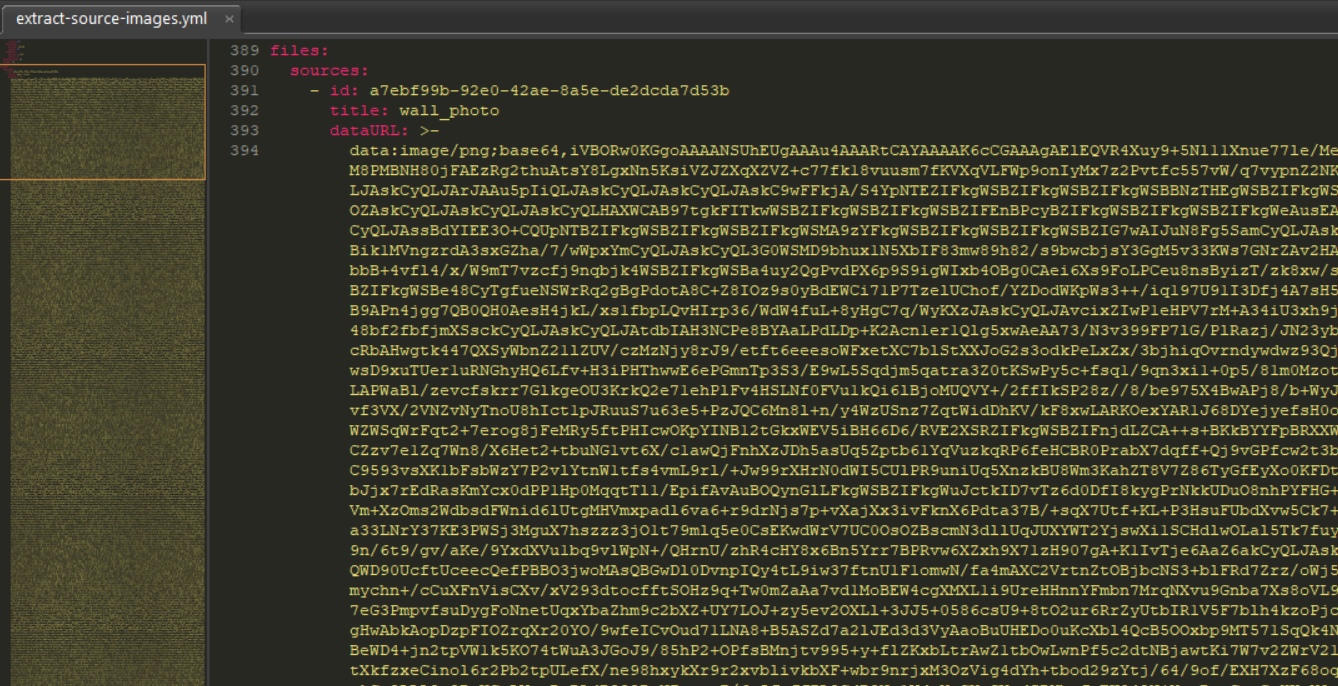
\includegraphics[width=1.0\textwidth]{sublime_1.PNG}

The path to this information looks like this:

files - sources - (unnamed) - dataURL

\itemizederror{Unnamed directory?}
{\item When figuring out the path to tell the function to follow in order to extract the image, I notice an empty space where I expect a directory name. Brian explains that this means this is an unnamed directory that exists in order to store an undefined number of sub-files (ie. the images). In order to incorporate this into a file path, we need to use a `for loop.'}

We also create a variable to incorporate into the For Loop that will parse all the YAML files, rather than just the one (there are three in the data folder)

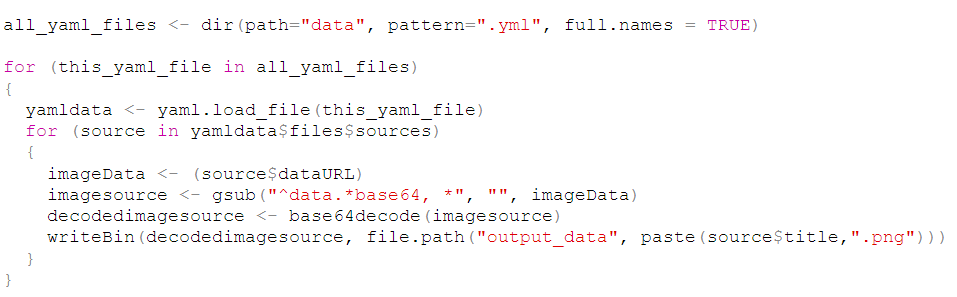
\includegraphics[width=1.0\textwidth]{rstudio_50.PNG}

When running this script, all YAML files are parsed in RStudio, then the dataURL that contains the information for the PNG files is extracted, the head of the dataURL is removed, as it is not needed, then what is left is decoded from Base64 (I downloaded the base64enc package for this), then written as a PNG file into the output\_data folder.

\textbf{Result}: Script for extracting source images from YAML files runs successfully and outputs the PNG files to the output\_data folder.

\subsubsection{Compare Gardiner Codes}

\textbf{Intention}: Develop R script that can isolate a series of pieces of information identified as `Gardiner Codes' and assign these values to variables that can be compared one to one and the exact matches calculated in order to determine what percentage the aotu-classify tool got correct.

\textbf{Actions}: To prepare for this code, I created two YAML (.yml) files from the HI Workbench, both with the same selection of hieroglyphic signs, but one I manually classified myself and the other I let the program auto-classify them. I call them \textit{Correct Gardiner Codes} and \textit{Incorrect Gardiner Codes}.

At first, I work on parsing the YAML files, isolating the Gardiner Codes, which are contained within an unnamed directory like above, and write them to separate text (.txt) files.

The code looks like this:

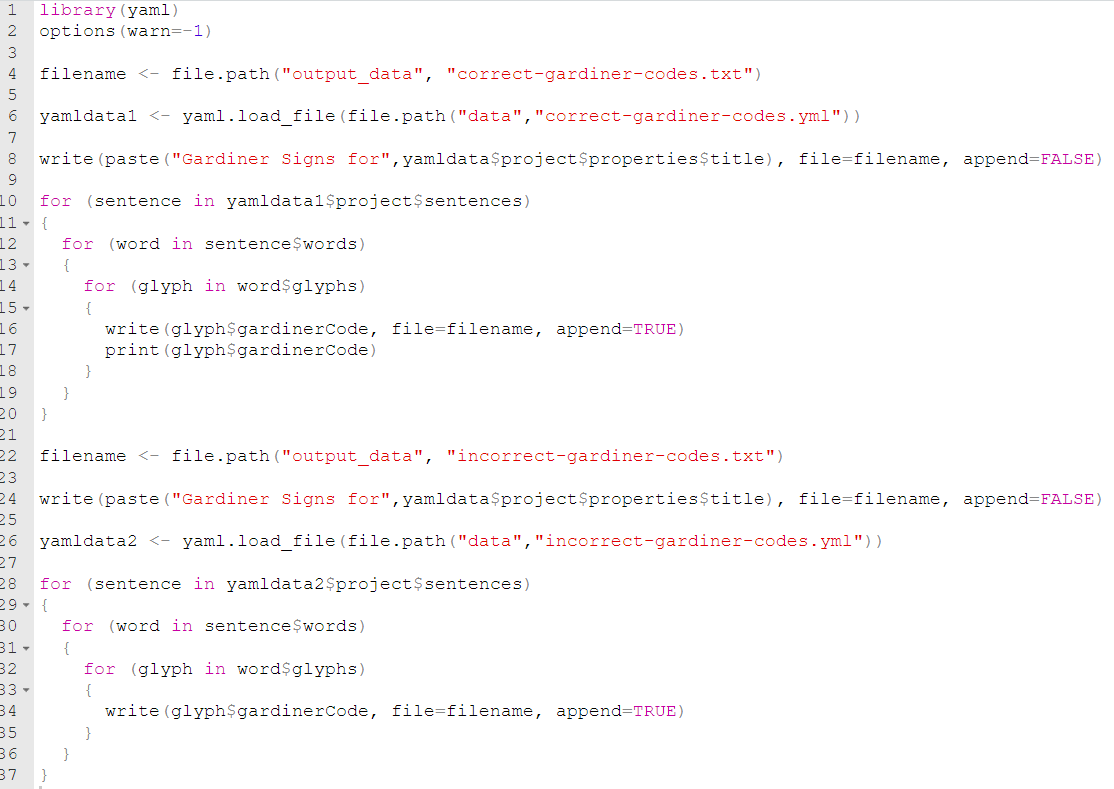
\includegraphics[width=1.0\textwidth]{rstudio_52.PNG}

When run, it successfully outputs two text files with the Gardiner Codes listed within them. Okay, cool...now what?

\itemizederror{How do I compare two .txt files?}
{\item I got a bit stuck when it came to actually comparing the two lists of Gardiner Codes.
\item Would I need to assign the contents of the two txt files to vectors, then compare them line by line?
\item How would I removed the first line, which is just a heading?}

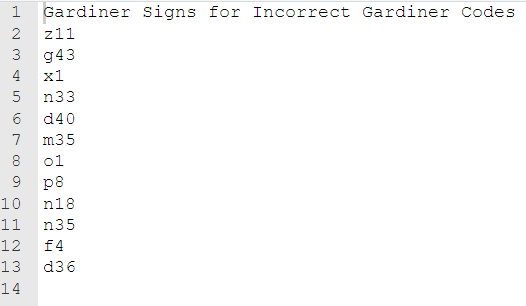
\includegraphics[width=1.0\textwidth]{rstudio_51.PNG}

I figured outputting the lists to txt files was a bit unnecessary and started working on extracting the Gardiner Codes using For Loops and assigning them to vectors in one go. See below:

\underline{Calculate Number of Records}:

\begin{minted}[breaklines]{R}
yamldata1 <- yaml.load_file(file.path("data","incorrect-gardiner-codes.yml"))

NumberOfRecords <- 0

for (sentence in yamldata1$project$sentences)
{
  for (word in sentence$words)
  {
    for (glyph in word$glyphs)
    {
      NumberOfRecords <- NumberOfRecords + 1
    }
  }
}
print(NumberOfRecords)
\end{minted}

\underline{Parse and Vectorise First File}:

\begin{minted}[breaklines]{R}
DataVector1 <- vector("character", length = 0)

for (sentence in yamldata1$project$sentences)
{
  for (word in sentence$words)
  {
    for (glyph in word$glyphs)
    {
      DataVector1 <- c(DataVector1, glyph$gardinerCode)
    }
  }
}
print(DataVector1)
\end{minted}

\underline{Parse and Vectorise Second File}:

\begin{minted}[breaklines]{R}
yamldata2 <- yaml.load_file(file.path("data","correct-gardiner-codes.yml"))
DataVector2 <-vector("character", length = 0)

for (sentence in yamldata2$project$sentences)
{
  for (word in sentence$words)
  {
    for (glyph in word$glyphs)
    {
      DataVector2 <- c(DataVector2, glyph$gardinerCode)
    }
  }
}
print(DataVector1)
print(DataVector2)
\end{minted}

\underline{Count Exact Matches in Files 1 and 2}:

\begin{minted}[breaklines]{R}
Count <- 1
MatchCount <- 0

while (Count <= NumberOfRecords)
{
  
  if(DataVector1[Count] == DataVector2[Count])
  {
    MatchCount <- MatchCount + 1
  }
  print(DataVector1[Count])
  print(DataVector2[Count])
  print(Count)
  print(MatchCount)
  Count <- Count + 1
}
\end{minted}

\underline{Calculate Percentage of Correct Matches}:

\begin{minted}[breaklines]{R}
PercentMatch <- MatchCount/NumberOfRecords*100
print(format(PercentMatch, digits=2, nsmall=2))
\end{minted}

I included \mintinline{R}|print| functions throughout so I could keep tabs on everything that is happening as the script runs. I used a \mintinline{R}|while| function instead of a For Loop for the Count, as I tried a For Loop, but could not get it to work the way I wanted it to, so I switched to something new and it worked how I wanted it, so I went with that. I got the script to give the outcome as a percentage (which came out as 25.00. The auto-classify function got 3 out of the 12 hieroglyphic signs...oh dear. Oh well, not the focus of the project at hand. The code works!)

\subsubsection{Unit Testing my Code}

\textbf{Intention}: Develop R script to test that the two R scripts that I have developed run as expected and give the expected output. To do this, I have to learn how to use the \mintinline{R}|testthat| package to create functions that tailor to specific script functions. (I learned this from Brian).

\textbf{Actions}: Following these two pages/sites:

\begin{verbatim}
https://towardsdatascience.com/unit-testing-in-r-68ab9cc8d211

https://cran.r-project.org/web/packages/testthat/testthat.pdf?
fbclid=IwAR07Bud7-Zkp9C-2np4B_TtlhR3cEtotpOlPUISUQDjl5vlOOVU6n
pqWuPo
\end{verbatim}
%https://cran.r-project.org/web/packages/testthat/testthat.pdf?fbclid=IwAR07Bud7-Zkp9C-2np4B_TtlhR3cEtotpOlPUISUQDjl5vlOOVU6npqWuPo

and with help from Brian and my dad, I develop a function that is supposed to test that the file path is followed and a vector is generated. (I also install the \mintinline{R}|testthat| package for this to work)

\begin{minted}[breaklines]{R}
library(testthat)

test_filename <- "incorrect-gardiner-codes.yml"

count_NumberOfRecords <- function(filename)
  {
  yamldata <- yaml.load_file(file.path("data",filename))
   NumberOfRecords <- 0
   for (sentence in yamldata$project$sentences)
   {
     for (word in sentence$words)
     {
       for (glyph in word$glyphs)
       {
         NumberOfRecords <- NumberOfRecords + 1
       }
     }
   }
   
  return(NumberOfRecords)
}

count_NumberOfRecords(test_filename)

test_that("create vector", expect_equal(count_NumberOfRecords("incorrect-gardiner-codes.yml"), 12))
\end{minted}

I run this script then run the following code in a new script file:

\begin{minted}[breaklines]{R}
test_file("scripts/Unit-Testing-Code.R")
\end{minted}

The test function returns this:

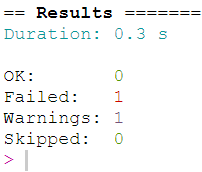
\includegraphics[width=0.5\textwidth]{rstudio_54.PNG}

\textbf{Result}: The test failed, but the rubric says I only have to attempt the unit testing, and I did give it a go, despite my lack of knowledge.

\section{Friday November 1st 2019}

\subsection{Setting up Code Ocean}

\subsubsection{Establishing Environment}

\textbf{Intention}: Set up environment within Code Ocean capsule to exactly match that of my working directory for my Proof of Concept R project.

\textbf{Actions}: Going into the `environment' tab in the capsule, I add the necessary packages (\mintinline{R}|yaml|, \mintinline{R}|base64enc|, and \mintinline{R}|testthat| (I initially forgot this one, but picked up on it later))

\textbf{Result}: Environment set up.

\subsubsection{Organising Files}

\textbf{Intention}: Place the necessary files (ie. R scripts, .yml files) in the appropriate directories within the Code Ocean capsule.

\textbf{Actions}: I upload the git repository for my Proof of Concept R project into the capsule, and copy the 4 R scripts into the `codes' directory, and the 3 .yml files into the `data' directory.

\textbf{Result}: Files organised into appropriate directories within my Code Ocean capsule.

\subsubsection{Reproducible Run}

\textbf{Intention}: Run the code with the environment set up and see if everything runs successfully.

\textbf{Actions}: I click the Reproducible Run button.

\itemizederror{Cannot open connection}
{\item I try to run the code after establishing Extract-Image-Files.R (or so I thought) as the main code to run, clicking the Reproducible Run button.
\item Some of the code runs alright, but I can see that part of the code is halted due to the error 'Cannot open connection'
\item I try changing up the file path in Extract-Source-Images.R, replacing ``data" with ``../data", ``./data"; ``..", ``data"; ``.",``data". 
\item Still getting the error.
\item I consult Brian on the matter over Slack, and he points out that the main code the Reproducible Run runs is actually Extract-Gardiner-Codes.R, so changing the file path in the Extract-Source-Images.R file wouldn't fix the problem.}

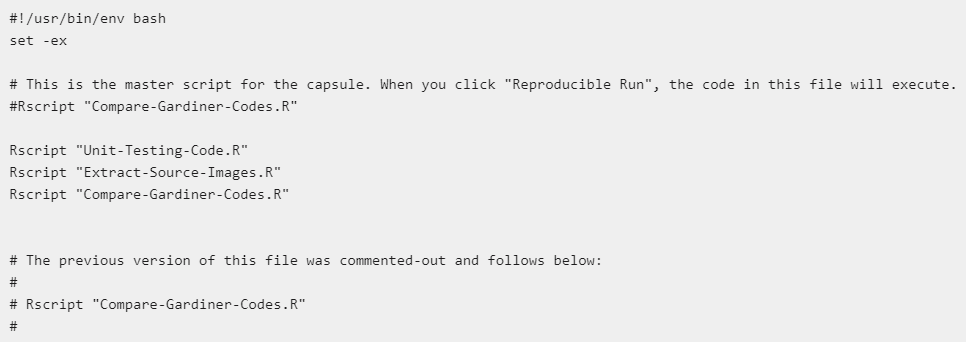
\includegraphics[width=1.0\textwidth]{rstudio_55.PNG}

Brian explains to me that Code Ocean has a specific style of writing file paths, which was something I had noticed when looking for help here:

\begin{verbatim}
    https://help.codeocean.com/en/articles/1082877-paths
\end{verbatim}

I change the order of the R scripts to:
\\Commpare-Gardiner-Codes.R

Extract-Source-Images.R
\\Unit-Testing-Code.R
\\Unit-Testing-Code\_test\_file.R

because I'm pretty sure the first Unit Testing script needs to be run before the other one for them to actually work. I could be wrong, but again. I tried.

\textbf{Result}: Code Ocean Capsule nearly complete. I try to click Submit for Publication, but it is telling me I haven't completed all of the necessary steps. Apparently I need to fill out more metadata information before I can submit.

\subsubsection{Submit for Publication}

\textbf{Intention}: Submit capsule for verification and then publication in order to complete process and then include in final project.

\textbf{Actions}: After filling in the required metadata fields, including author name, subject field, and a short description, I click the Submit for Publication button.

\itemizederror{5 Business Days to Verify}
{\item I notice that I do not have the option to Share my capsule and thus cannot generate a url intended to be shared online.
\item I notice at the top of my Workspace, it says that my capsule is still being verified. I Google how long this process usually takes.
\item Apparently it can take up to 5 business days. Which means my capsule may not be published until Friday. This project is due a 2pm on Saturday, and I am working all day on Saturday.
\item I message Brian asking for his advice. As I have already shared access to my capsule with the Collaborate function of the site, he should be able to access it even while it is in the middle of the verification process.
\item I send him the link again just to double check and he states that it works. Good enough, I suppose.}

\textbf{Result}: Code Ocean capsule complete and ready to be added to Proof of Concept project.

\section{Saturday November 2nd 2019}

\subsection{Completing Proof of Concept Project}

\textbf{Intention}: Finish off the final few things I need to do in order to complete my Proof of Concept project. I have completed the R scripts now, and just need to finish the Read Me file, the Acceptance Tests file (which tells you how to use the Code Ocean capsule), and then that should be it.

\textbf{Actions}: Using the GitHub interface, I edit the ReadMe file so that it includes instructions on how to follow the Code Ocean link, run the code (using the Acceptance Tests file), and how to generally navigate the repository (including a note that the version control history is actually in the other repository called Proof-of-Concept rather than Proof-of-Concept\_Final).

\textbf{Result}: Git Repository complete and ready for marking. Learning Journal complete and ready for marking. Exporting as .pdf and uploading in 3..2..

\end{document}